\chapter{Fuels} 
\label{ch:fuels}

Fuel for wildland fire consists of vegetation. 
Recall from Eq.~\ref{eq:combustion} that combustion is essentially the decomposition of plant matter\textemdash originally produced by photosynthesis\textemdash in the presence of oxygen and sufficient heat. 
Because a high degree of variability in fire behavior can be attributed to variability in fuels, making good fuel measurements is essential to predicting how a prescribed fire will burn and explaining variability in the effects that fire produces. 

\section{Broad considerations}

\subsection{Fuels and the fire regime}

The primary consideration of fire regime in planning fuels measurement is identifying the \emph{fire type} by determining which vegetation layer(s) carries the fire (Fig.~\ref{fig:ParametersFactors}). 
Under all but the most extreme conditions in densely-wooded vegetation, prescribed fire management is typically focused on surface fires that consume herbaceous vegetation rooted in\textemdash or laying on\textemdash the soil surface. 
\footnote{Note that in woodlands and savannas, the fuelbed often contains leaf litter that fell from tree canopies, which are considered surface fuels once they have fallen.}

Next, one must determine if live fuel is a consideration (we assume here that it is). 
How to determine if live fuels are relevant? 
Consider the conditions below. 
If any apply to a burn or study, one should likely be measuring live and dead fuels separately: 

\paragraph{Checklist for live fuel relevance} 
\begin{itemize}[noitemsep]
	\item[{\color{BisonGreen!80}\ding{51}}] Prescription for growing season burn
	\item[{\color{BisonGreen!80}\ding{51}}] Vegetation dominated by exotic cool-season (C\textsubscript{3}) grasses
	\item[{\color{BisonGreen!80}\ding{51}}] Management and/or research objectives focus on any C\textsubscript{3} grass
	\item[{\color{BisonGreen!80}\ding{51}}] Research objectives include parameterizing custom fuel models and/or modeling fire behavior  
\end{itemize}

However, if none of the above conditions apply, one is probably not missing out on much information by not dividing the fuelbed up into live and dead components.

There are two basic types of information on fuels the fire scientist ought to obtain \emph{by fuel class}\footnote{While these would typically also be described by size class, in the workshop we are considering only 1 hr fuels, so we will consider each in terms of live and dead components.}: 

\begin{itemize}[noitemsep]
	\item Fuel load 
	\item Fuel moisture
\end{itemize}

\subsection{Sampling approaches}

There are two broad categories of sampling methodologies, each with pros and cons specific to wildland fuel sampling, although the pros and cons likely apply to other sampling contexts, as well: 
\begin{itemize}
	\item \textbf{Destructive\textemdash}Samples are collected by physically removing material from the environment. 
	\begin{itemize}[noitemsep]
		\item[\textit{Pros:}]Most accurate; probably needs fewest observations. Raw data in desired units (mass/area for fuel load, \% $H_{2}O$ for fuel moisture).
		\item[\textit{Cons:}]Removes from the fire environment the very thing one seeks to describe within the fire environment. 
		Time consuming. 
		Requires weighing and drying equipment.
		Data not instantaneously available. 
	\end{itemize}
	\item \textbf{Non-destructive\textemdash}Sampling consists of observations that do not require the material to be disturbed. 
		\begin{itemize}[noitemsep]
		\item[\textit{Pros:}]Doesn't remove any fuel from the fire environment. Most often requires less sample processing time \& effort, and data can be instantaneously available. 
		\item[\textit{Cons:}]Likely requires more observations to minimize variability. Raw data rarely on a meaningful scale; often needs a conversion factor that in turn must often be derived from separate calibration efforts.
	\end{itemize}
\end{itemize}

Whether one implements destructive or non-destructive sampling has profound implications on the nature of the sampling protocol and the data it produces, including the transferability of data to other events and locations and even whether the data are useful for the stated purposes. 
Consider just a few examples of how different wildland fire professionals might need different types of data on different time scales: 
\begin{itemize}
	\item \emph{The burn boss wants to make tactical decisions on fuel conditions such as a minimum or maximum fuel load, or minimum dead fuel moisture.} 
	They will need this information the day of the burn\textemdash they cannot wait for samples to be clipped, dried for 48 h, and weighed. 
	On the other hand, an estimation based on a representative but limited sample is probably sufficient. 
	The values likely do not need to be applied to other locations. 
	\item \emph{The biologist has designed a monitoring program to assess shrub mortality across several sites with different amounts of smooth brome.} 
	Whether that smooth brome was green or not at the time of the fire\textemdash and how much of it there was\textemdash is likely important information. 
	On the other hand, categorical assessments of live:dead biomass based on non-destructive observations is probably sufficient.
	An estimation of live fuel moisture based on a representative but limited sample would probably be icing on the cake. 
	\item \emph{A graduate student has a hypothesis that connects fire behavior to fuel parameters.} 
	It is important that multiple pre-fire measurements be taken around each fire behavior observation point, and continuous variables are best. 
	On one hand, statistical analysis can take fuel load on any scale, so a rapid, non-destructive quantification method will be fine.
	On the other hand, reviewers are likely going to want to be able to connect these data to actual values, and managers will need those values to apply the findings well, so it is best to have a plan for calibration. 
	An accurate measure of fuel moisture is important, but the data aren't needed until well after the fire, so there is plenty of time to dry and weigh clipped samples. 
\end{itemize}  

These questions help guide a responsive and informative sampling plan: 

\begin{itemize}[noitemsep]
	\item[] \hspace{-1.9em}\emph{Ask first:}
	\item[{\color{BisonGreen!80}\ding{51}}]\emph{Who} is expecting the data and \emph{what} are they going to use it for?
	\item[{\color{BisonGreen!80}\ding{51}}]\emph{When} are they expecting it?
	\item[] \hspace{-1.9em} \emph{Then determine:}
	\item[{\color{BisonGreen!80}\ding{51}}]\emph{What} will be reported
	\item[{\color{BisonGreen!80}\ding{51}}]\emph{How and when} data will be collected 
\end{itemize}

\section{Measuring fuel load} 

\subsection{Destructive sampling}

Clipping is the most straightforward form of measuring fuel load in grasslands. 
A representative sample point is identified, a known area determined, and all vegetation\textemdash representing combustible fuel\textemdash is removed by hand and stuffed into a paper bag (Fig.~\ref{fig:clipping}). 
Once dried and weighed, the mass of the material in the bag is easily expressed as the fuel load for the known area from which the sample was collected.

\begin{figure*} 
		\begin{center}
	\includegraphics[width=0.57\textwidth]
		{science/Fuels/ClippingQuadratShears}~
	\includegraphics[width=0.43\textwidth]
		{science/Fuels/DryGrassBag}
			\end{center}
	\caption{On the left, a 0.25 m\textsuperscript{-2} quadrat is about to be clipped with sheep shears (this might sound silly, but they are the secret weapon for efficient grass clipping). 
		Once bagged, the samples are dried in a forced air drying oven at at least 60\degC{ }for at least 48 h. 
		After drying, samples are weighed and their mass expressed on a per-area basis.
		 } \label{fig:clipping}
	%(Fig.~\ref{fig:clipping})
\end{figure*}

\paragraph{Clipping} 

Clip all material to within about 2 cm or 1 inch of the soil surface. 
The main idea is to gather as much combustible material as possible while being as consistent from sample to sample. 
Clipping and scraping right down to bare mineral soil when one can will produce a different picture of the available fuel load than a quadrat with a thicker mat of wet litter that is unlikely to burn anyway. 
Better to be consistent from quadrat to quadrat. 
Deposit clipped material in a paper bag clearly labeled with a marker. 

%\begin{marginfigure}
%	\begin{center}
%		\includegraphics[width=2.2in]
%		{science/fuels/residue}
%		\caption{Even a hot fire can't burn it all off. 
%			\label{fig:residue} } 
%		% (Fig.~\ref{fig:residue})
%	\end{center}
%\end{marginfigure}

\paragraph{Drying}

Clipped biomass samples are typically dried in forced-air ovens at at least 60\degC.\footnote{There is debate around the minimum temperature required to adequately dehydrate samples, although differences have the most effect on determining moisture content, not dry mass. 
	Thus this debate is discussed in the fuel moisture section below.}
The aim is to dehydrate clipped biomass to the point that the samples reach an equilibrium moisture content with the air in the oven\textemdash as the weight of samples at such a state would no longer loose mass, complete drying of samples is often referred to as ``constant mass.``
With herbaceous samples, this often occurs within 48 hours. 
 
\paragraph{Weighing}

Weigh dried biomass samples on a digital balance shortly after removal from the oven, before they absorb moisture from the cooler ambient air. 
The primary concern with weighing is accounting for the mass of the paper bag. 
One can either dump the bag contents into a tared container on the balance, or weigh the sample in the bag and subtract the mass of the bag. 
There are many arguments for the latter\textemdash it is often faster and less messy\textemdash but it is prone to error if different types of bags are used. 
A best practice for data management is to enter a code for the bag type when entering mass data for each sample, or group of samples with a common bag type, and assign the mean mass of several empty bags to each code when subtracting bag weights prior to analysis.

\subsection{Nondestructive sampling}

Nondestructive sampling of fuel load\textemdash i.e., measurements taken without physically removing material from the fuelbed\textemdash has several distinct advantages. 
Chiefly, nondestructive sampling leaves the fuelbed intact, which ensures that the amount of fuel recorded in the data is actually the amount of fuel available to burn. 
If too many clipping samples are taken from too small of an area around a fire behavior sensor, the removal of fuel could reduce intensity and rate of spread.  
Fire behavior data from that sensor would not represent the rest of the fire. 

The most common technique for non-destructive sampling of aboveground vegetation in North American rangeland is known as the Robel pole (Fig.~\ref{fig:RobelPole}). 
Initially presented by \citet{robel1970}, the point was to make a measurement that combined the height and density of prairie vegetation to assess wildlife habitat.
The pole itself was 3 cm in diameter, 150 cm long, and painted in 1 dm (10 cm) increments. 
Observers stood the pole upright in the vegetation, stepped back 4 m, and bent down such that eye level was 1 m. 
The lowest increment on the pole that was 50\% obscured by vegetation was recorded; this came to be known as the \emph{visual obstruction reading}, or VOR. 

	
\begin{figure*}[!b]
		\caption{Two views of a Robel pole in place: Left, in very low biomass due to repeated grazing following a patch burn; Right, in tall, fully-headed out smooth brome grass in an idled CRP field.
	} 
	\begin{center}
		\includegraphics[width=0.36\textwidth]
		{science/Fuels/RobelPoleShort}~
		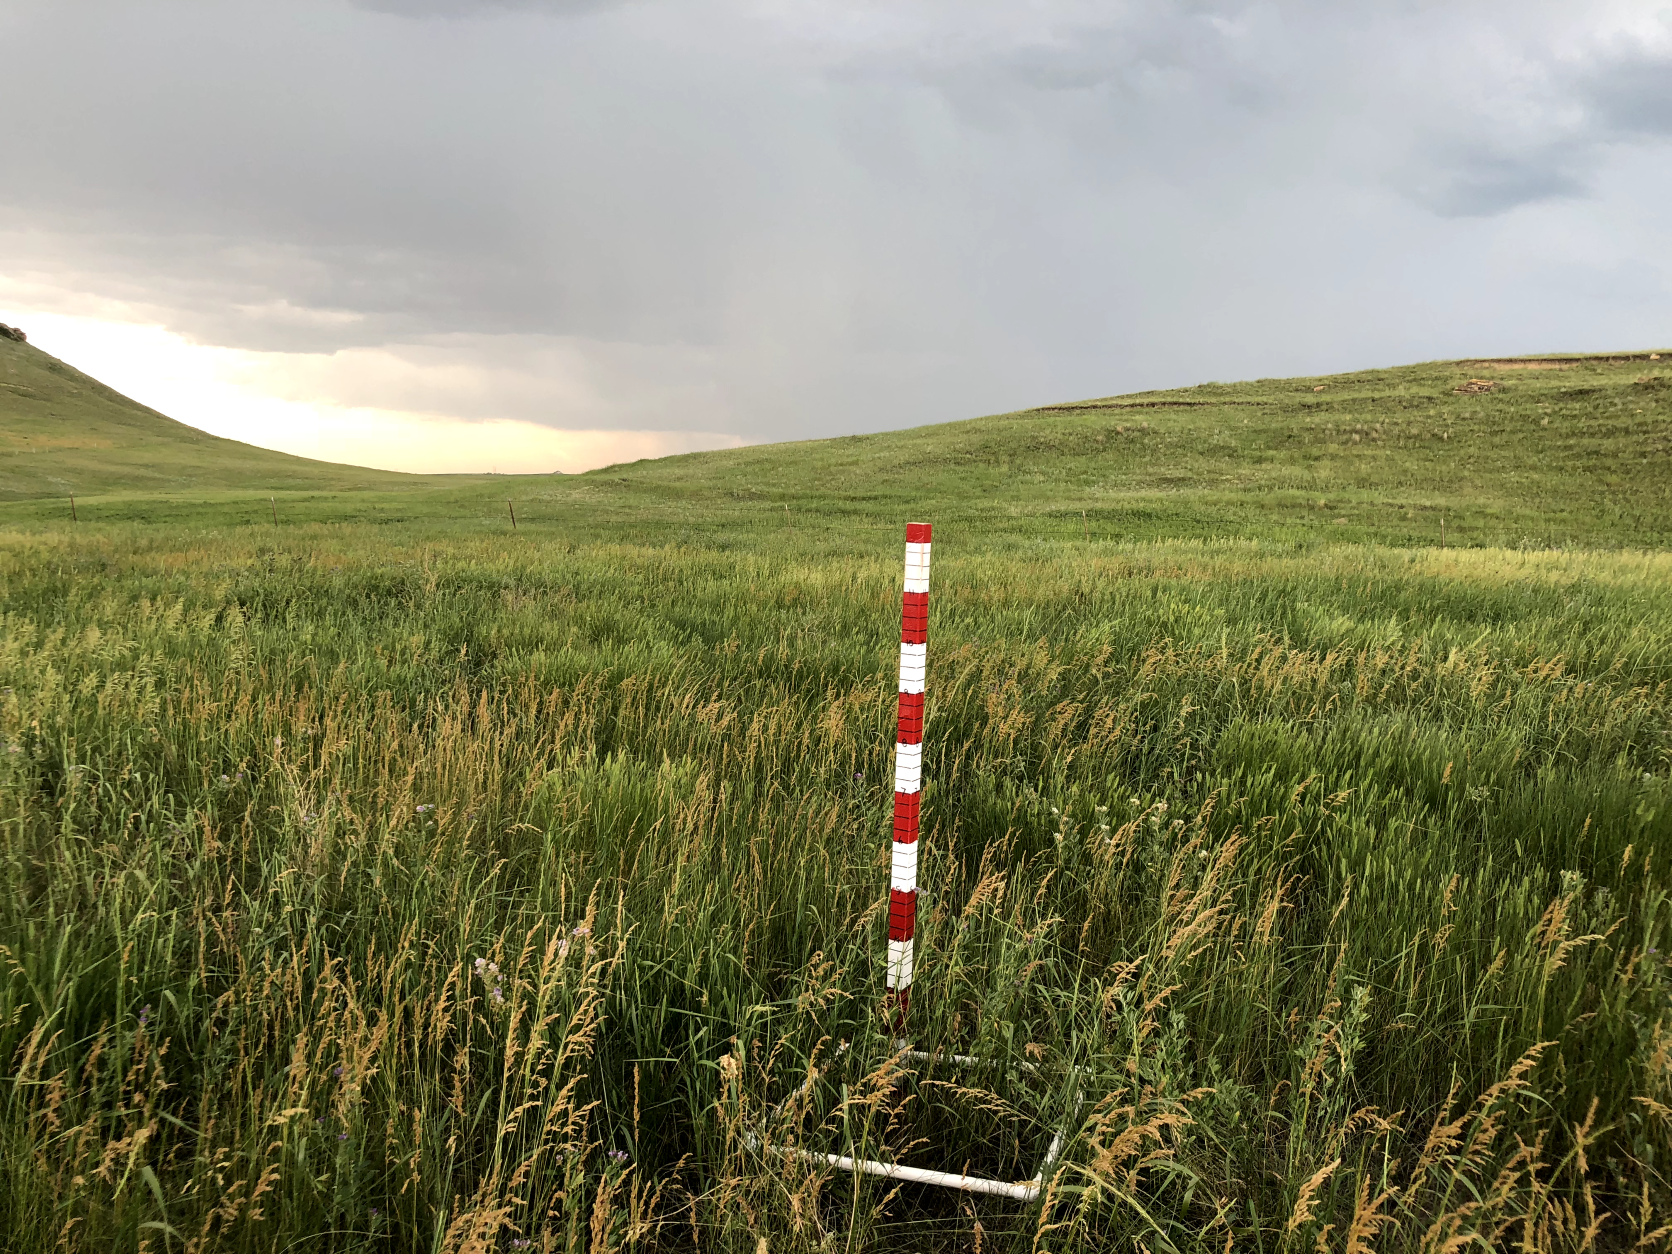
\includegraphics[width=0.64\textwidth]
		{science/Fuels/RobelPoleBrome}
	\end{center}
\label{fig:RobelPole}
	%(Fig.~\ref{fig:RobelPole})
\end{figure*}

Crucially, the VOR had ``a striking relationship between the visual obstruction measurements and the weight of vegetation clipped from each transect \citep[][p. 296]{robel1970}.''
From their analysis of data averaged at the transect level,\footnote{Standard practice has become to collect four VOR measurements around each pole placement, typically from the four cardinal directions, and average those readings for a single observation. This works well for fuel load measurements around fire behavior sensors not oriented along transects.} the relationship between the non-destructive VOR measured from the Robel pole and actual vegetation biomass (g m\textsuperscript{-2}) could be well explained ($R^2 = 0.97$) by the linear relationship 

\begin{equation}\label{eq:robel1}
\text{biomass}_{g~m^{\text{-}2}} =  113 \cdot \text{VOR}_{dm} + 1.9
\end{equation}

The utility of VOR in estimating herbaceous biomass has been confirmed several times since the Robel pole was introduced. 
Two studies in particular compared VOR to other non-destructive methods, and found it to be the most accurate in both hayfield/pasture situations and native rangeland \citep{harmoney1997, ganguli2000}. 
\citet{vermeire2002} fit a new linear equation to a combined dataset from shortgrass, mixed-grass, and tallgrass prairie (1000-7000 kg ha\textsuperscript{-2}; $R^2 = 0.93$):

\begin{equation}\label{eq:robel2}
	\text{biomass}_{kg~m^{\text{-}2}} =  183 \cdot \text{VOR}_{cm} + 538
\end{equation}

While they note that users can get better accuracy by creating location-specific calibration equations by comparing VOR measurements to their own clipped quadrats, this general equation provides a good estimate across grasslands in general. 

\subsection{Differentiating fuel components} 

Often information is needed on specific parts of the fuelbed. 
When live fuels are a consideration, live and dead components must be assessed separately. 
Managers and researchers are often interested in litter separate of the total fuel load. 
Below are approaches for each. 

\subsubsection{Live vs. dead}

The most accurate method to report live and dead components of the fuel load are to measure each separately. 
``Hand sorting'' is the process of placing live and dead fuel in their own bags for separate weighing. 
Samples can be sorted as they are clipped, or prior to drying; the sooner it occurs, the easier it is to distinguish live material from dead. 

But hand sorting is very time-consuming, and fortunately alternative methods have been developed. 
The \emph{constituent differential method} from \citet{gillen1993} uses known values of wet weight (mass in the field, just after clipping) and dry weight (mass after drying) for pure sub-samples of live and dead biomass to determine the fractions of each in combined samples.
When fuel samples are clipped on the same day as a burn, the pure sub-samples of live and dead fuel can also be used for fuel moisture measurements.

Live:dead fractions can also be estimated via visual categorization. 
This is a more rapid technique that does not require any clipping from the fuel load, although its accuracy can be improved via calibration with clipping data from a local stand similar to the fuelbed. 
Visual categorization based on color tends to over-predict curing, because fuels start to \emph{look} cured before their moisture content has actually gotten below the moisture of extinction \citep{kidnie2015}. 

\subsubsection{Litter} 

\paragraph{Destructive sampling}
Perhaps the best way to measure litter separately when clipping plots is to clip all standing plant material down to the top of the litter layer\textemdash not to within 3 cm of the soil surface right away\textemdash then collect the litter into a separate bag. 
Any remaining standing material can then be clipped to 3 cm of the soil surface and added to the first bag.

\begin{marginfigure}
	\begin{center}
		\includegraphics[width=2.2in]
		{science/fuels/MeasuringLitterDepth}
		\caption{Measuring litter depth with a ruler. \label{fig:LitterRuler} } 
		% (Fig.~\ref{fig:LitterRuler})
	\end{center}
\end{marginfigure} 

\paragraph{Non-destructive sampling} 
Specific litter depth measurements can be made with a ruler (Fig.~\ref{fig:LitterRuler}). 
Do not rely on a separate reading on a Robel pole, which is likely too coarse\textemdash in terms of both the diameter of the pole pushing down litter, and the width of the increments\textemdash to provide a sufficiently precise measurement. 
Find an average of multiple depth readings taken from a focal area (e.g., a quadrat). 
Then, if necessary, additional work can likely be done to calibrate the average depth to biomass on a per-area basis. 

  
\section{Measuring fuel moisture} 

As with fuel load, the most reliable measurements of fuel moisture content are made by clipping physical samples. 
There are two differences to consider when clipping for fuel moisture samples: Less material is needed, making it less disruptive to the overall fuelbed, and fuel moisture samples must be weighed before drying as well as after. 
Critically, \emph{the pre-drying mass should be taken as soon after clipping as possible}, to prevent moisture loss (Fig.~\ref{fig:GreenBalance}). 
If samples are at risk of going for more than an hour or so before pre-drying mass can be determined, they should be handled in sealed, non-permeable containers like zippered baggies or bottles and kept out of direct sunlight and hot environments until they can be weighed. 

 \begin{marginfigure}
	\begin{center}
		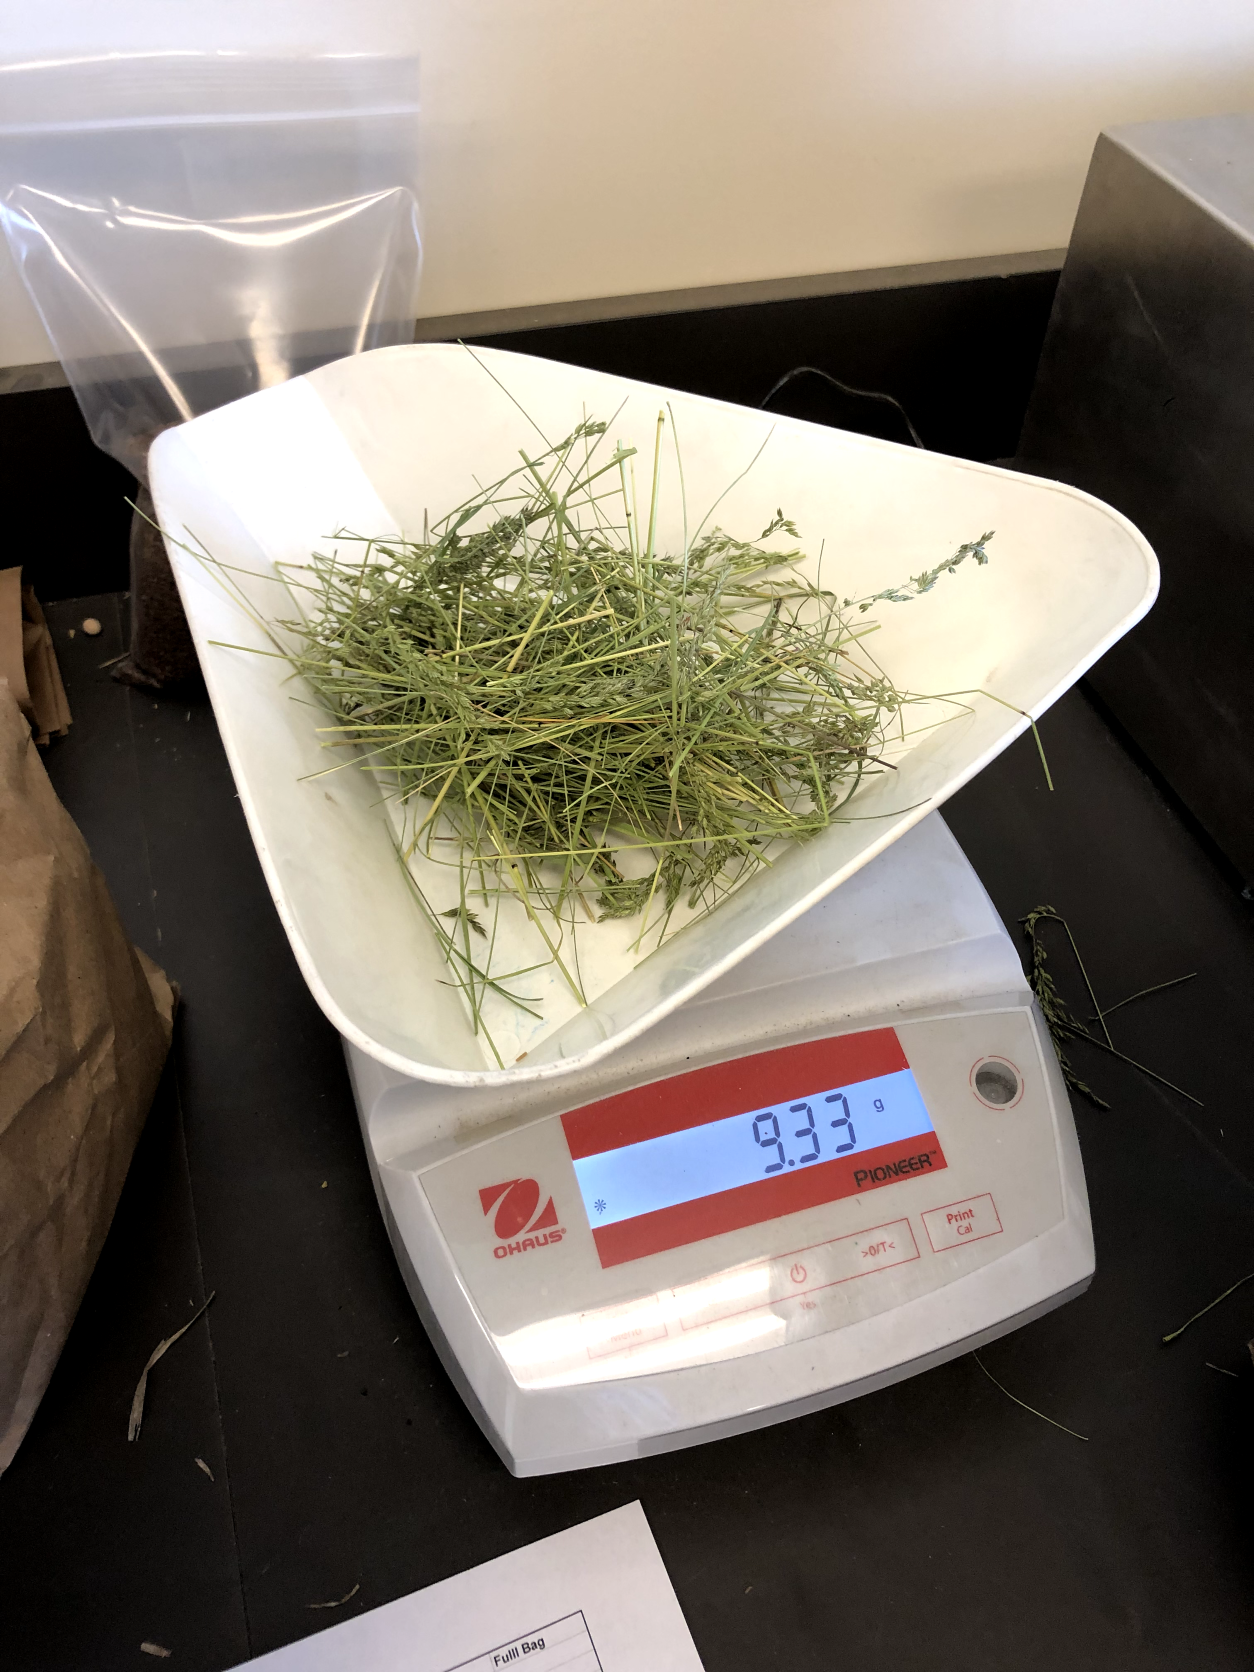
\includegraphics[width=2.2in]
		{science/fuels/LiveFuelsBalance}
		\caption{Green, live grass material is weighed separately prior to drying. \label{fig:GreenBalance} } 
		% (Fig.~\ref{fig:GreenBalance})
	\end{center}
\end{marginfigure}

There is debate around the best temperature to sufficiently dry samples intended for fuel moisture measurement.
On one hand, \citet{gillen1993} only set their drying ovens to 45\degC; this is likely too low to be recommended for measuring fuel moisture content.
\citet{matthews2010} compared the moisture content of dead grass fuels after 48 h in ovens set at 60\degC{ } and 105\degC, and found they averaged 10\% and 8\% moisture, respectively, which could be a meaningful difference if, for example, dead fuel moisture is being used as an input for fire behavior calculations.\footnote{For example, a BehavePlus calculation for tallgrass prairie (fuel model 3) that assumes a 10 mph wind on flat ground indicates fire will spread 8 m min\textsuperscript{-2} faster at 8\% fine dead fuel moisture than at 10\% (83 vs. 75 m min\textsuperscript{-2}, respectively).}
On the other hand, further work suggests drying temperature is less important, given the amount of variability inherent among samples, especially for live fuels \citep{jolly2011}. 

If day-of fuel moisture measurements are required, there are a few options. 
Firstly, smaller sample volumes can be sufficiently dehydrated in a microwave oven to get a reasonable estimation of fuel moisture. 
Secondly, there are technologies that use electricity to determine the moisture content of plant material\textemdash many such devices are used in the grain industry, for example, to monitor moisture content.  
Campbell Scientific manufactured a moisture meter specifically for wildland fuels (Fig.~\ref{fig:dmm}), but unfortunately only a limited number were produced and new units are not available.

\begin{figure*}
	\caption{The Campbell Scientific DMM-600 duff moisture meter uses electricity to instantaneously determine the moisture content of a sample. 
		In addition to forest duff, it is effective for live fuel moisture in grassland fuels \citep{mcgranahan2019}.
		Unfortunately the manufacturer's website indicates the product has been retired.
	} 
	\begin{center}
		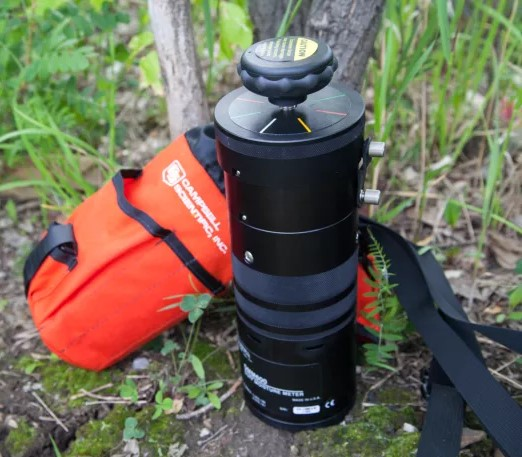
\includegraphics[width=0.46\textwidth]
		{science/fuels/dmm}~
		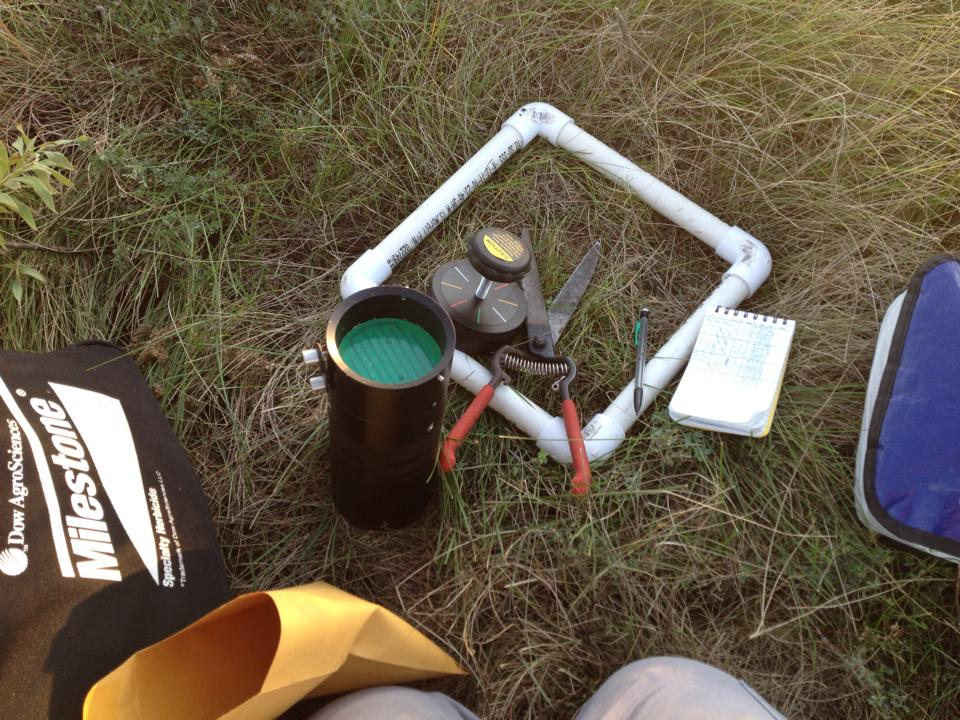
\includegraphics[width=0.54\textwidth]
		{science/fuels/clipping}
	\end{center}
	\label{fig:dmm}
	%(Fig.~\ref{fig:dmm})
\end{figure*}
